\graphicspath{{./chapitres/chapitre8/figures/}}
\setcounter{mtc}{8}
\chapter{Sprint Six : Déploiement de l'application}
\minitoc
\newpage
\section*{Introduction}
Au sixième chapitre nous avions parlé du l'architec déploiement de l'application et de la configuration technologique.
Il étale par la même occasion la procédure du déploiement de l'application et la configuration technologique.

\section{Conception architecturale}
\subsection{Architecture g\'en\'erale}
Cette section est consacr\'ee \`a d\'eterminer et d\'elimiter la vision globale de l'architecture technique \`a mettre en \oe uvre. 

En effet, d'apr\`es les exigences fonctionnelles \'etudi\'ees, notre solution fera n\'ecessairement l'objet d'une application Web. Le support du Web s'av\`ere le plus ad\'equat pour les applications complexes d\'elivr\'ees \`a partir d'une infrastructure centralis\'ee pour des clients l\'egers. 

Notre application Web repose sur une architecture trois-tiers (Client l\'eger-Serveur d'application-Serveur de base de donn\'ees).

L'architecture globale est introduite par la figure \ref{fig:architecture} qui montre explicitement le principe de la s\'eparation des trois niveaux suivants :
\begin{itemize}
\item La pr\'esentation des donn\'ees : Il s'agit d'un client l\'eger qui \'etablit une communication avec un serveur d'application et lance une requ\^ete afin d'obtenir un r\'esultat tangible souhait\'e.
\item La Logique m\'etier (le traitement m\'etier des donn\'ees) : c'est le niveau qui prend en charge la mise en \oe uvre de l'ensemble des r\`egles de gestion et de la logique applicative. Un serveur d'application s'occupe de traiter les requ\^etes reçues par le client et de lui renvoyer une r\'eponse.
\item Les donn\'ees : ce troisi\`eme et dernier niveau concerne les donn\'ees persistantes qui sont destin\'ees \`a \^etre acc\'ed\'ees et utilis\'ees par notre application. Ces donn\'ees sont conserv\'ees sur la dur\'ee, voire de mani\`ere d\'efinitive. Le serveur de base de donn\'ees reçoit des requ\^etes de la part du serveur d'application et consulte la base de donn\'ees derri\`ere pour restituer les donn\'ees demand\'ees (ou bien effectuer toute autre op\'eration de manipulation de donn\'ees).
\end{itemize}
\begin{figure}[!ht]\centering
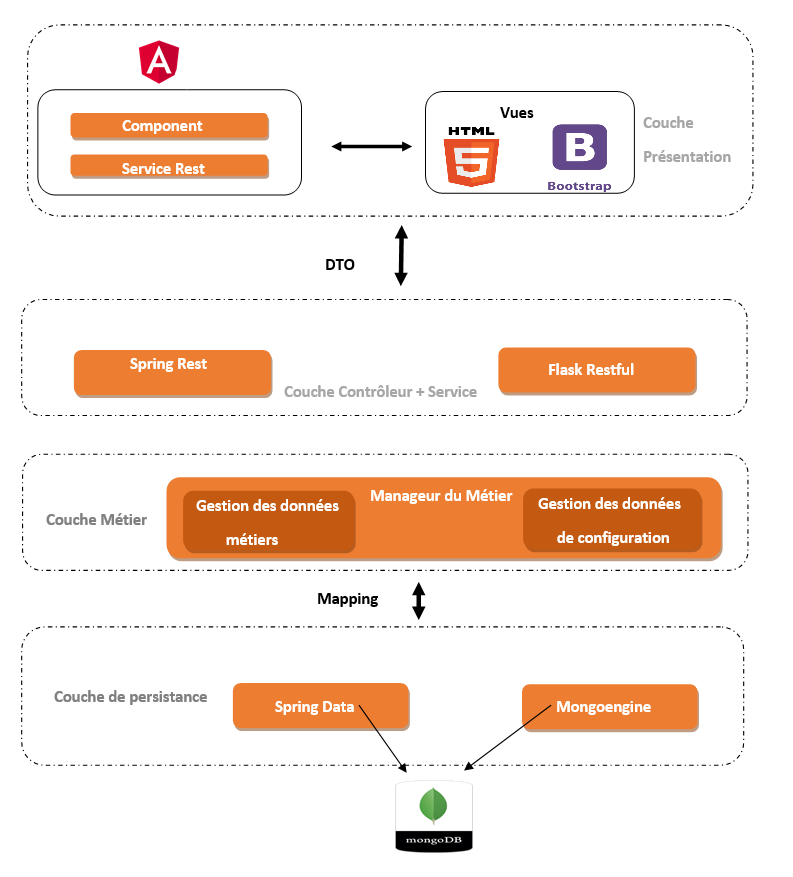
\includegraphics[scale=0.8]{architecture}
\caption{Architecture globale}
\label{fig:architecture}
\end{figure}

\subsection{Architecture d\'etaill\'ee}

L'architecture de notre application se caract\'erise par les couches suivantes :
\subsubsection*{La couche Pr\'esentation (Couche Web)}
Cette couche s'occupe des interactions directes avec l'utilisateur final (le client l\'eger) ; nous y trouvons des \'el\'ements tels que : des contr\^oleurs, des gestionnaires d'utilisateurs, des groupes, des r\^oles, des fonctionnalit\'es, et dans
notre cas la sous-couche DTO (Data Transfer Object).
\paragraph{La couche DTO}
Cette couche sert \`a d\'eplacer les donn\'ees vers et à partir de la couche de pr\'esentation. Id\'ealement, ceci se fait \`a travers la cr\'eation d'objets qui sont utilis\'es pour transmettre des donn\'ees \`a partir de la couche de pr\'esentation \`a la couche Services, et inversement. Un objet de transfert de donn\'ees (DTO) d\'etient toutes les donn\'ees qui sont nécessaires pour l'appel distant d'une des couches Présentation et Services.

\subsubsection*{La couche Logique M\'etier}
Cette couche constitue le c\oe ur du m\'etier ; c'est \`a dire le traitement (aspect fonctionnel et op\'erationnel transform\'e \`a partir de la sp\'ecification des besoins) derri\`ere l'application. Elle renferme elle-même plusieurs sous-couches. Les
contr\^oleurs de la couche Pr\'esentation acc\`edent \`a cette couche (plus pr\'ecis\'ement \`a travers la sous-couche "Services").
\paragraph{La couche contrôlleurs}
Cette couche permet d'exposer, comme son nom l'indique, des services exploitables par des tierces parties (Couche Pr\'esentation). C'est l'impl\'ementation des r\'egles de gestion m\'etier.
\paragraph{La couche DAO/Acc\`es aux Donn\'ees}
Les objets d'acc\`es aux donn\'ees (DAOs) se comportent r\'eellement comme une couche d'abstraction des donn\'ees (physiques)
pour les couches Entit\'es et Services. Ils se chargent de la manipulation des entit\'es en requ\^etant directement le serveur de base de donn\'ees et s\'eparent les acc\`es donn\'ees requis par l'application, en termes d'objets m\'etier sp\'ecifiques et de types de donn\'ees.
\paragraph{La couche Entit\'es}
Celle-ci regroupe toutes les entit\'es et les classes de mapping correspondant aux donn\'ees persistantes (tables) de la base de donn\'ees. Elle n'est accessible qu'au niveau de la couche Services et la couche DAO. Cette isolation permet d'affaiblir \'enorm\'ment le couplage entre ces objets et les \'el\'ements de la couche Pr\'esentation.
\subsubsection*{La Couche Infrastructure}

\paragraph{La couche Configuration}
Celle-ci permet de d\'efinir des configurations de certains \'el\'ements configurables de l'application (la couche web, la couche s\'ecurit\'e et la couche DAO par exemple) \`a des fins diff\'erentes. Elle contient des classes de configuration
ainsi que des fichiers de propri\'et\'es.

\section {Diagramme de déploiement}
La figure \ref{fig:DeploymentDiagram1} présente le diagramme de déploiement de notre solution.  

\begin{figure}[!ht]\centering
\fbox{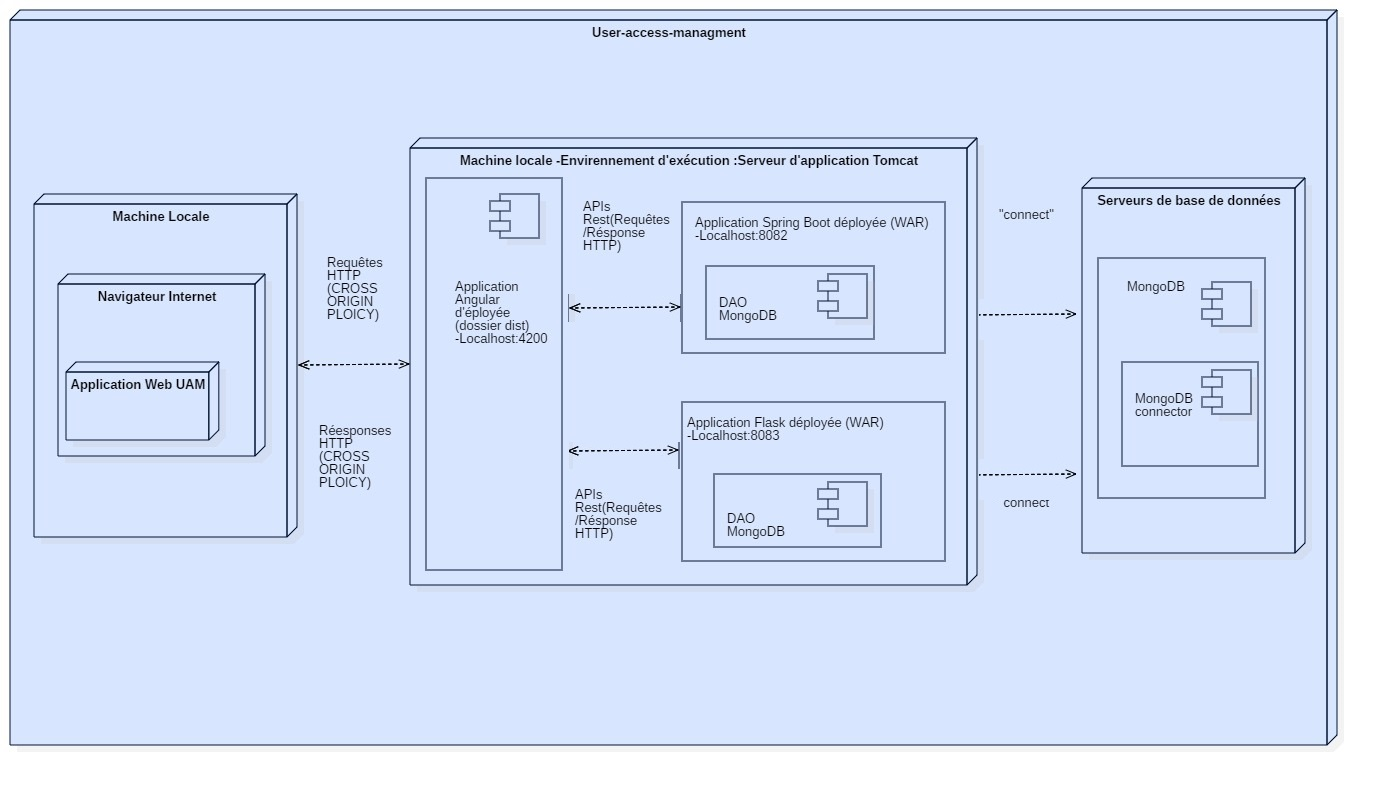
\includegraphics[width=1\columnwidth]{chapitres/chapitre8/figures/DeploymentDiagram1.jpg}}
\caption{Diagramme de déploiement : architecture physique}
\label{fig:DeploymentDiagram1}
\end{figure}

\section{Environnement de travail}
\subsection{Environnement logiciel}
\subsubsection*{Apache Tomcat 9}
Tomcat est un serveur d'applications Java. Nous avons déjà présenté ce qu'est une application web. Elle permet de générer une réponse HTML à une requête après avoir effectué un certain nombre d'opérations (connexion à une base de données, à un annuaire LDAP...). Pour le client (un navigateur web en général), il n'y a pas de différence avec une page web statique : il reçoit toujours du HTML, seul langage qu'il comprend. Seule la manière dont la réponse est formée côté serveur change.
\begin{figure}[!ht]\centering

\includegraphics[width=0.4\textwidth]{chapitres/chapitre8/figures/apachtomcat.png}
\caption{Apache Tomcat logo}
\label{fig:apachtomcat}
\end{figure}
\section{Accès à l'application monitoring des transactions }	
L'accès au l'application monitoring des transactions sera matérialisé par un lien web sur l'onglet "Identification du client". Il sera accessible en vue normale si le CA souhaite regarder les dernières transactions de son client et en vue KYC.

Depuis CBS, il conviendra de matérialiser l’accès à ce dashboard par un mécanisme similaire.

Lors de la revue KYC, le chargé d'affaires devra impérativement avoir revu les transactions pour pouvoir valider le KYC. Dans le cas où la revue n'a pas été effectuée, un message s'affichera : 

"Avant de valider l'authentification de l'acteur, vous devez vérifier le profil de transactions de de ses clients, accessible via le lien "l'application monitoring des transactions".
\newline
La figure suivante présente une interface de CRM modifier à cause de confidentialités et cette interface présente le scénario de l'accès à notre application
\newpage
\begin{figure}[!ht]\centering
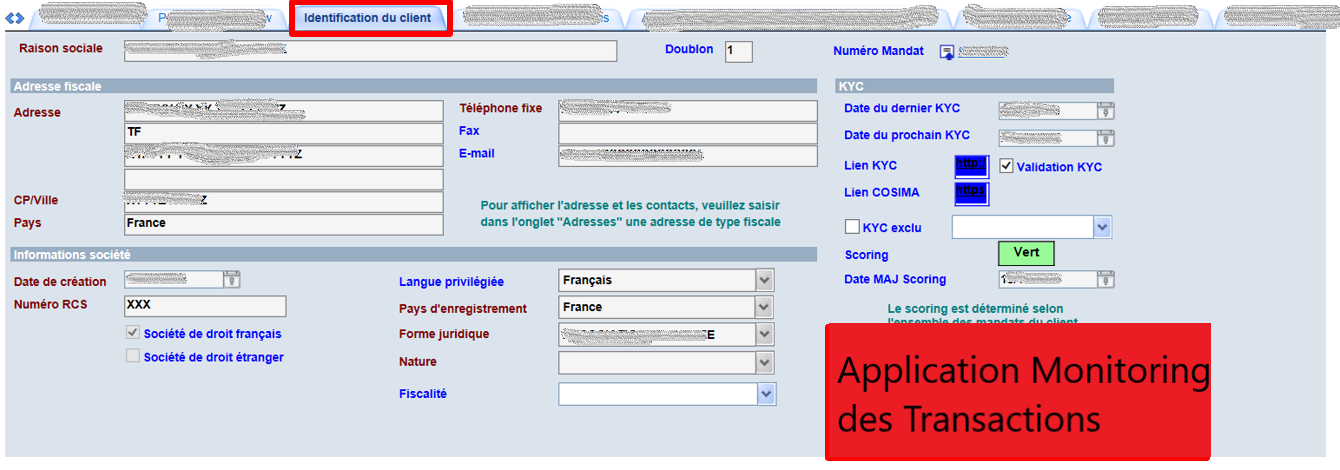
\includegraphics[width=1\textwidth]{chapitres/chapitre8/figures/acces.png}
\caption{Accès à l'application monitoring des transactions}
\label{fig:acces}
\end{figure}
\section*{Conclusion}
Au cours de ce chapitre nous avons présenté et argument\'e notre architecture et la structure générale pour mise en place notre application.